\documentclass{article}
\usepackage{aligned-overset}
\usepackage{amsmath}
\usepackage{amssymb}
\usepackage{bm}
\usepackage[shortlabels]{enumitem}
\usepackage{hyperref}
\usepackage[utf8]{inputenc}
\usepackage{mathtools}
\usepackage{physics}
\usepackage{tabularx}
\usepackage{titling}
\usepackage{fancyhdr}
\usepackage{xfrac}
\usepackage{pgfplots}

\definecolor{light-gray}{gray}{.9}

\pgfplotsset{compat = newest}

\author{Karsten Lehmann}
\date{SoSe 2021}
\title{Übung 02 Analysis - Weiterführende Konzepte}

\pagestyle{fancy}
\fancyhf{}
\lhead{\thetitle}
\rhead{\theauthor}
\lfoot{\thedate}
\rfoot{Seite \thepage}

\begin{document}

\section*{Existenz von Stammfunktionen}

Untersuchen Sie, ob folgenden Aussagen wahr oder falsch sind:

\begin{enumerate}[a)]
\item Jede Funktion $f \in R([a, b])$ besitzt auf $[a, b]$ eine Stammfunktion.

  \textit{Lsg.} Diese Aussage ist falsch.

  \textbf{Beweis mit Gegenbeispiel:}
  \begin{itemize}
  \item $f(x) = \frac{1}{x}, I = [a, b], 0 \notin I$.
    In diesem Fall ist $f$ stetig und beschränkt, somit ist
    $F(x) = \int_a^x f(t) \,dt$ die Stammfunktion $\Rightarrow$ das ist kein Gegenbeispiel
  \item $f = \begin{cases}
      0 & x = 0 \\
      \frac{1}{x} & x \ne 0 \\
    \end{cases}, I = [0, 1]$
    In diesem Fall ist $f$ nicht beschränkt, somit ist $f \notin R([0, 1])$
    $\Rightarrow$ das ist kein Gegenbeispiel
  \item $f = \begin{cases}
      1 & x \in [0, 1] \\
      -1 & x \in [-1, 0) \\
    \end{cases}, I = [-1, 1]$

    \begin{tikzpicture}
      \begin{axis}[
        axis lines=middle,
        xmax = 1.5,
        xmin = -1.5,
        ymax = 1.2,
        ymin = -1.2,]
        \addplot [
        domain=0:1,
        samples=100,
        very thick, blue]{1};
        \addplot [
        domain=-1:0,
        samples=100,
        very thick, blue]{-1};
      \end{axis}
    \end{tikzpicture}
  \end{itemize}

  $\Rightarrow f \in T([0, 1]) \subseteq R([0, 1])$

  $F(x) = \int_0^x f(t) \,dt = \begin{cases}
    x & x \in [0, 1] \\
    -x & x \in [-1, 0) \\
  \end{cases} = \abs{x}$

  $F$ ist auf $[-1, 1]$ nicht differenzierbar, da $f'(0)$ nicht existiert.

  $F_1(x) = x, x \in \underset{I_1}{\underbrace{[0, 1]}},
  F_2(x) = -x, x \in \underset{I_2}{\underbrace{[-1, 0]}}$.
  Dabei ist $F_1$ ist eine Stammfunktion auf $I_1$ und $F_2$ eine Stammfunktion
  auf $I_2$.
  Allerdings ist $F(x) = \begin{cases}
    F_1(x) & x \in I_1 \\
    F_2(x) & x \in I_2 \\
  \end{cases}$ keinen Stammfunktion auf $I_1 \cup I_2$.

  \fcolorbox{black}{light-gray}{
    \begin{minipage}{\textwidth}
      \textbf{Satz von Darboux} (Zwischenwertsatz für Ableitungen)
      
      Sei $I \in \mathbb{R}$ ein Intervall und $f \colon I \to \mathbb{R}$
      eine Differenzerbare Funktion, dann

      \[
        \forall c \in \left( \inf_{x \in I} f'(x) , \sup_{x \in I} f'(x) \right)
        \exists \eta \in I \colon f'(\eta) = c
      \]
    \end{minipage}
  }

  Aus dem Satz von Darboux folgt: Sprungfunktionen besitzen niemals Stammfunktionen.

  $\Rightarrow$ Funktionen mit einem Sprung, wie zum Beispiel $f(x) = sgn(x)$
  widerlegen die Aussage.

  
\item Ist $f$ auf $[a, b]$ differenzierbar, so ist $f'$ auf $[a, b]$ Riemann-integrierbar.

  \textit{Lsg.} Diese Aussage ist falsch.

  $f(x) = \begin{cases}
    x^2 \sin\left(\frac{1}{x^2}\right) & 0 < \abs{x} < 1 \\
    0 & x = 0 \\
  \end{cases}$

  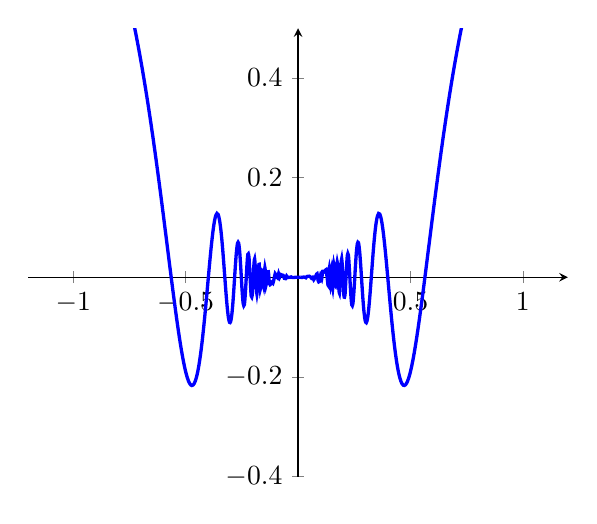
\begin{tikzpicture}
    \begin{axis}[
      axis lines=middle,
      xmax = 1.2,
      xmin = -1.2,
      ymax = 0.5,
      ymin = -0.4,]
      \addplot [
      domain=0.01:1,
      samples=200,
      smooth,
      very thick, blue]{x^2 * sin(deg(1 / x^2))};
      \addplot [
      domain=-1:0.01,
      samples=200,
      smooth,
      very thick, blue]{x^2 * sin(deg(1 / x^2))};
    \end{axis}
  \end{tikzpicture}

  
  \begin{align*}
    \Rightarrow x \ne 0 \colon f'(x) &= 2x \sin\left(\frac{1}{x^2}\right) + x^2 \cos\left(\frac{1}{x^2}\right)\left(-\frac{2}{x^3}\right) \\
                                     &= 2x \sin\left(\frac{1}{x^2}\right) - \colorbox{yellow}{$\frac{2}{x} \cos\left(\frac{1}{x^2}\right)$} \\
    x = 0 \colon f'(x) &= \lim_{h \to 0} \frac{f(h) - f(0)}{h} = \lim_{h \to 0} \frac{h^2 \sin\left(\frac{1}{h^2}\right)}{h} \\
                                     &= \lim_{h \to 0} h \cdot \underset{\abs{\ldots} \leq 1}{\underbrace{\sin\left(\frac{1}{h^2}\right)}} = 0 \\
  \end{align*}

  In der Ableitung ist ein \colorbox{yellow}{Ausdruck}, der dafür sorgt, dass diese nicht beschränkt ist.
  Sei $x_k = \frac{1}{\sqrt{2k\pi}} \in (0, 1]$

  \begin{align*}
    f'(x_k) &= \frac{2}{\sqrt{2k\pi}} \underset{= 0}{\underbrace{\sin(2k\pi)}} - 2 \sqrt{2k\pi} \underset{= 1}{\underbrace{\cos(2k\pi)}} \\
            &= - 2 \sqrt{2k\pi} \overset{k \to \infty}{\longrightarrow} -\infty
  \end{align*}
  
\end{enumerate}

\section*{Integration mittels Substitution}

Ermitteln Sie größtmögliche Intervalle $I \in \mathbb{R}$ auf denen die
folgenden Ausdrücke $f(x)$ Stammfunktionen besitzen.
Berechnen Sie zugehörige Stammfunktionen $F \colon I \to \mathbb{R}$
durch Anwendung des Hauptsatzes.

\begin{enumerate}[a)]
\item $f(x) = \frac{6}{1 - 3x}$
\item $f(x) = 3 \sqrt{8x - 4}$
\item $f(x) = \frac{1}{\sqrt[3]{5x - 7}}$
\item $f(x) = \frac{x}{4 + x^2}$
\item $f(x) = \frac{2x + 4}{x^2 + 4x + 7}$
\item $f(x) = \frac{x^2}{x^3 - 27}$
\item $f(x) = \frac{1}{x \cdot \ln x}$
\item $f(x) = 3e^x \sqrt{e^x + 1}$
\item $f(x) = \cos(x) \sin(2x)$
\end{enumerate}

\section*{Integration mittels Substitution oder partieller Integration}

Ermitteln Sie größtmögliche Intervalle $I \in \mathbb{R}$ auf denen die
folgenden Ausdrücke $f(x)$ Stammfunktionen besitzen.
Berechnen Sie zugehörige Stammfunktionen $F \colon I \to \mathbb{R}$
durch Anwendung des Hauptsatzes.

\begin{enumerate}[a)]
\item $f(x) = x (\sin x^2 + \cos x^2)$
\item $f(x) = x^2 \sin x$
\item $f(x) = \exp\left( a \sqrt{x} + b \right), a \ne 0$
\item $f(x) = (x^2 -  4) \cos(2x)$
\item $f(x) = \frac{x^3 + 4x}{(x^2 + 4)^2}$
\item $f(x) = \exp(ax) \cos(bx), a, b \ne 0$
\end{enumerate}

\section*{Rekursionsformeln}

Stellen Sie für die folgenden Integrale
$F_n (x) \coloneqq \int_0^x f_n(t) \,dt, x \in \mathbb{R}$ und
$n \in \mathbb{N}_0$ Rekursionsformeln auf.
Geben Sie explizite Darstellungen von $F_0, \ldots, F_3$ an.

\begin{enumerate}[a)]
\item $f_n(t) = t^n e^{at}, a \ne 0$
\item $f_n(t) = \sin^n(t)$
\end{enumerate}

\end{document}